\documentclass{beamer}
\usepackage{beamerthemeshadow}
\usepackage{verbatim}

\usepackage{lastpage}
\usepackage{xcolor}
\usepackage{pgf}
\usepackage{colortbl}
\usepackage{hyperref}
\usepackage{multirow}

\usepackage{siunitx}
\sisetup{input-symbols=(), group-digits  = false} 

\newcommand{\bi}{\begin{itemize}}
\newcommand{\ei}{\end{itemize}}
\newcommand{\be}{\begin{enumerate}}
\newcommand{\ee}{\end{enumerate}}
\newcommand{\bd}{\begin{description}}
\newcommand{\ed}{\end{description}}
\newcommand{\prbf}[1]{\textbf{#1}}
\newcommand{\prit}[1]{\textit{#1}}
\newcommand{\beq}{\begin{equation}}
\newcommand{\eeq}{\end{equation}}
\newcommand{\bdm}{\begin{displaymath}}
\newcommand{\edm}{\end{displaymath}}

\newcommand{\ft}[1]{
  \frametitle{\begin{tabular}{p{4.2in}r} \textcolor{white}{#1} & \small{\insertframenumber / \inserttotalframenumber} \end{tabular}}
  \setbeamercovered{transparent=18}
}

\newcommand{\eft}[1]{
  \frametitle{\begin{tabular}{p{4in}r} \textcolor{white}{#1} & \small{\hyperlink{f:questions}{\beamergotobutton{GO BACK}}} \end{tabular}}
  \setbeamercovered{transparent=18}
}

\newcommand{\stepinv}{\setbeamercovered{invisible}}
\newcommand{\stopinv}{\setbeamercovered{transparent=18}}
\newcommand{\uncoverinv}[1]
{
  \setbeamercovered{invisible}
  \uncover<+->{#1}
  \setbeamercovered{transparent=18}
}
\newcommand{\ans}[1]{\textcolor{blue}{#1}}
\newcommand{\ansinv}[1]
{
  \setbeamercovered{invisible}
  \uncover<+->{\textcolor{blue}{#1}}
  \setbeamercovered{transparent=18}
}
\newcommand{\setinv}{\setbeamercovered{invisible}}
\newcommand{\setvis}{\setbeamercovered{transparent=18}}
\newcommand{\centerpic}[2]
{
  \begin{center}
  \includegraphics[#1]{#2}
  \end{center}
}
\newcommand{\h}[1]{\hat{#1}}
\newcommand{\ds}{\displaystyle}

\definecolor{light}{rgb}{1.0,0.7,0.7}
\definecolor{BrickRed}{rgb}{0.8,0.1,0.1}
%\definecolor{light}{rgb}{1.0,0.5,0.5}
\newcommand{\hl}[1]{\only<#1>{\cellcolor{light}}}

\definecolor{mycolor}{rgb}{0.6,0.0,0.0}
\usecolortheme[named=mycolor]{structure}

\title[Fiscal Policy Uncertainty and Macroeconomic Consequences]{Identifying Fiscal Policy Uncertainty and Its Macroeconomic Consequences}
\author[James Murray, University of Wisconsin - La Crosse]
{
James Murray\\
Department of Economics\\
University of Wisconsin - La Crosse
}
\date{August 2, 2014}

\begin{document}

\frame{\titlepage \setcounter{framenumber}{0}}

\frame
{
  \ft{Purpose}
  \begin{block}{Quantify uncertainty concerning fiscal policy}
    \bi
    \item Realistic framework for forming expectations
    \item Isolate five sources:
      \begin{tabular}{p{1.9in}p{2in}}\\ [-0.5pc]
      Government expenditures & Government debt \\
      Taxes & Overall fiscal uncertainty \\
      Transfers & \\
      \end{tabular}
    \ei
  \end{block}

  \begin{block}{Estimate the Macroeconomic Impact}
    \bi
    \item Autoregressive distributed lag (ARDL) models with fiscal uncertainty explanatory variables.
    \item Five dependent variables:
      \begin{tabular}{p{1in}p{1in}p{1in}}\\ [-0.5pc]
      Real GDP & Investment & Inflation \\
      Consumption & Unemployment & \\
      \end{tabular}
    \ei
  \end{block}
}

\frame
{
  \ft{Literature}
  \begin{block}{Time-varying Fiscal Volatility}
  \bi
  \item Fern\'andez-Villiverde et. al. (2011a): Fiscal policy uncertainty is stagflationary
  \item Born and Pfeifer (2011): 
    \bi
    \item Significant evidence for time-varying volatility in fiscal shocks.
    \item Not a significant driver for business cycles.
    \ei
  \item Johannsen (2012): Matters more at ZLB.
  \ei
  \end{block}

  \begin{block}{Other ways of doing it}
  \bi
  \item Baker, Bloom, and Davis (2013): Index based on headlines, variance of professional forecasts, expiring tax provisions.
  \item Orlik and Veldkamp (2013): 
    \bi
    \item Not about fiscal policy.  Macro uncertainty.
    \item Uncertainty is margin of error for forecasts.
    \item Forecasts are based on Bayesian learning and model uncertainty.
    \ei
  \ei
  \end{block}
}

\frame
{
  \ft{Literature}
  \begin{block}{Specific Fiscal Challenges}
    \bi
    \item Bi, Leeper, and Leith (2013): Time and composition of fiscal consolidations
    \item Davig, Leeper, and Walker (2010): Unsustainable entitlement programs
    \item Davig and Foerster (2013): Expiring tax provisions - with uncertain extensions.
    \item Richter and Throckmorton (2013): uncertain debt targets
    \ei
  \end{block}
}

\frame
{
  \ft{Constant Gain Learning}
  \begin{block}{Constant gain learning mechanism}
    \bi
    \item Every period, run a least-squares regression for each fiscal policy variable, using data from previous periods.
    \item Weighted least squares - more recent observations have more weight.
    \item Regression forecast serves as expectation.
    \item Root (weighted) mean squared error serves as \textit{fiscal policy uncertainty}.
    \ei
  \end{block}

 \begin{block}{Ideal situations for constant gain learning}
    \bi
    \item Precedence of structural changes
    \item No a-priori knowledge on menu or evolution of structural changes and probability distributions
    \item Forecasting rule, but no knowledge of parameter values, or the structure of the whole economy.
    \ei
  \end{block}

}

\frame
{
  \ft{Fiscal Policy Regressions}
  \begin{block}{Empirical Model for Fiscal Policy Behavior}
  Each fiscal policy variable ($f_{i,t}$) responds to:
  \bi
  \item Lag of all fiscal policy variables ($f_{t-1}$).
  \item Above includes lag of government debt ($b_{t-1}$).
  \item Macro outcomes: real GDP ($y_t$), consumption ($c_t$), investment ($I_t$), and unemployment ($u_t$).
  \item All quantities real, per capita, ratio of past real GDP.
  \ei
  \end{block}

  \begin{block}{Four regressions}
  \textbf{Fiscal policy variables:} $f_{t} = [g_t~ r_t~ n_t~ b_t]$ \\ 
  Govt Spending ($g_t$), Tax Revenue ($r_t$),\\
  Net Transfers ($n_t$), Government Debt / GDP ($b_t$) \\ [0.5pc]

  \textbf{Regression equation:}\\
  $f_{i,t} = \alpha_{t,0} + \alpha_{t,f}' f_{t-1} + \alpha_{t,y} y_{t} + \alpha_{t,c} c_t + \alpha_{I,t} I_t + \alpha_{t,u} u_{t} + \epsilon_t$
  \end{block}
}

\frame
{
  \ft{Constant-Gain Learning}
  \begin{footnotesize}
  \begin{block}{Recursive Formulation}
    \bdm \begin{array}{c}
      \hat{\alpha}_{i,t} = \hat{\alpha}_{i,t-1} + \gamma R_t^{-1} X_t (f_{i,t} - X_t' \hat{\alpha}_{i,t}) \\ [1pc] 
      R_t = R_{t-1} + \gamma (X_t X_t' - R_{t-1}),
    \end{array}\edm
    \bi
    \item Learning gain, $\gamma \in (0,1)$, is constant, equal to the weight assigned to most recent observation.
    \item Typical estimates for $\gamma \sim 0.02$ (Milani (2008), Slobodyan and Wouters (2008)).
    \ei
  \end{block}

  \begin{block}{Standard Formulation}
    \bdm \hat{\alpha}_{i,t} = \left( (1-\gamma)  \sum_{\tau=1}^{t} \gamma^{\tau} X_{t-\tau} X_{t-\tau}' \right)^{-1}  \left( (1-\gamma)  \sum_{\tau=1}^{t} \gamma^{\tau} X_{t-\tau}  f_{i,t-\tau} \right). \edm
    Weight on $t-\tau$ observation declines geometrically with $\tau$: $\omega_\tau = (1-\gamma) \gamma^{\tau}$.
  \end{block}
  \end{footnotesize}
}

\frame
{
  \ft{Instrumental Variable (IV) Regression} 
  \begin{block}{Endogeneity Problem}
  \bi 
  \item Macro outcomes (real GDP, consumption, investment, and unemployment) are likely endogenous.
  \item Maybe market participants account for that.
  \item Use instruments: lags of macro outcomes and fiscal variables
  \ei
  \end{block}

  \begin{block}{Instrumental Variables Notation}
  \bi
  \item Let $W_{t} = [y_{t}~ c_t~ I_{t}~ u_{t}]'$ denote the possibly endogenous regressors in $X_{t}$,
  \item Let $V_{t} = [1~ f'_{t-1}]'$ denote the remaining exogenous regressors
  \item Then, $X_{t} = [V_t'~ W_{t}']'$.
  \item Let $S_t = [W'_{t-1}~ W'_{t-2}~ f'_{t-2} ]$ denote vector of instruments.
  \item Let $Z_t = [V'_t~ S'_t]'$ denote vector Stage 1 IV regressors.
  \ei
  \end{block}
}

\frame
{
  \ft{Two-Stage IV Least-Squares Learning}
  \begin{block}{Stage 1: Endogenous macro variable on instruments + exogenous}
    $W_{i,t} = Z_{t}' \beta_i + \upsilon_{i,t}$.\\[0.3pc]
    $\hat{\beta}_{i,t} = \hat{\beta}_{i,t-1} + \gamma \left(R_t^{S1}\right)^{-1} Z_{t-1} \left(W_{i,t-1} - Z_{t-1}'\hat{\beta}_{i,t-1}\right)$ \\ [0.3pc]
    $R_t^{S1} = R_{t-1}^{S1} + \gamma \left(Z_{t-1} Z_{t-1}' - R_{t-1}^{S1}\right)$ 
  \end{block}

  \begin{block}{Save Stage 1 Predicted Values}
  $\hat{W}_{i,t} = Z_{t}' \hat{\beta}_{i,t},~~~  \hat{X}_t = [V_t'~ \hat{W}_t']'$
  \end{block}

  \begin{block}{Stage 2: Constant Gain Learning with IV}
    $\hat{\alpha}_{i,t}^{IV} = \hat{\alpha}_{i,t-1}^{IV} + \gamma \left(R_t^{S2}\right)^{-1} \hat{x}_{t-1} \left(f_{i,t-1} - \hat{X}_{t-1}'\hat{\alpha}_{i,t-1}\right)$ \\ [0.3pc]
    $R_t^{S2} = R_{t-1}^{S2} + \gamma \left(\hat{X}_{t-1} \hat{X}_{t-1}' - R_{t-1}^{S2}\right)$. 
  \end{block}
}

\frame
{
  \ft{Fiscal Policy Uncertainty}
  \begin{block}{Unexplained fiscal policy at time $t$}
    Model prediction error:
    \bdm \epsilon_{i,t} = f_{i,t} - \hat{\alpha}_{i,t}^{IV'} X_t \edm
    \bi
    \item $\hat{\alpha}_{i,t}^{IV'}$ captures information in past fiscal policy behavior
    \item $X_t$ captures \textit{current} macroeconomic conditions.
    \ei
  \end{block}
  \begin{block}{Fiscal uncertainty measure}
    Root (weighted) mean squared error:\\
    \bdm m_{i,t}^{IV} = \sqrt{ (1-\gamma) \ds \sum_{\tau=1}^{t} \gamma^{\tau} \epsilon_{i,t}^2} \edm
  \end{block}
}

\frame
{
  \ft{Forecast Uncertainty vs. Time-Varying Volatility}
  \begin{block}{Time-Varying Volatility}
  \bi
  \item Eg: Fern\'andez-Villiverde et. al. (2011), Born and Pfeifer (2011), Johannsen (2012), etc.
  \item Can separate causal effects of fiscal shocks from i.i.d. innovations to variance.
  \item Possibly unrealistic set of knowledge and perceptions.
  \item Is fiscal policy uncertainty exogenous?
  \ei
  \end{block}

  \begin{block}{Model Prediction Uncertainty}
  \bi
  \item Agents are learning fiscal policy processes.
  \item Constant gain learning: accounts for structural change possibility.
  \item Fiscal shocks can move expectations away from true model.
  \item Time-varying uncertainty need not depend on time-varying volatility.
  \ei
  \end{block}
}

\frame
{
  \ft{Prediction Uncertainty}
  \begin{block}{Some basis in the literature:}
    \bi
    \item Herro and Murray (2013): Monetary policy uncertainty.
    \item Orlik and Veldkamp (2013): Macro uncertainty - forecast uncertainty with Bayesian learning
    \ei
  \end{block}
  \begin{block}{Shortcomings}
    \bi
    \item Learning models do not consider government budget constraint
    \item Backward looking - ignores policy announcements, upcoming policy expiration
    \item Long-horizon fiscal problems.
    \ei
  \end{block}
 }

\frame
{
  \ft{Fiscal Policy - Actual and Predicted}
  \begin{tabular}{cc}
    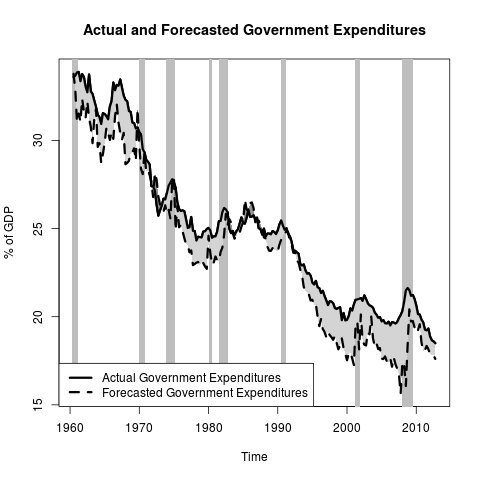
\includegraphics[width=0.45\textwidth, height=0.45\textheight]{pics/pred_gov.png} & 
    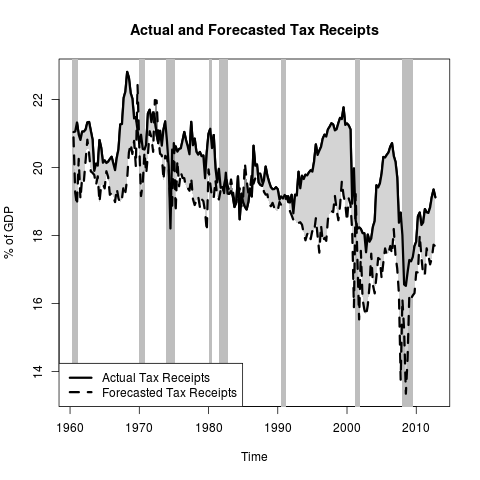
\includegraphics[width=0.45\textwidth, height=0.45\textheight]{pics/pred_tax.png} \\ 
    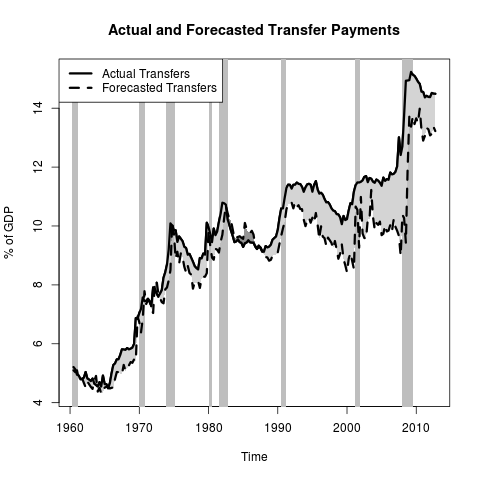
\includegraphics[width=0.45\textwidth, height=0.45\textheight]{pics/pred_transfers.png} & 
    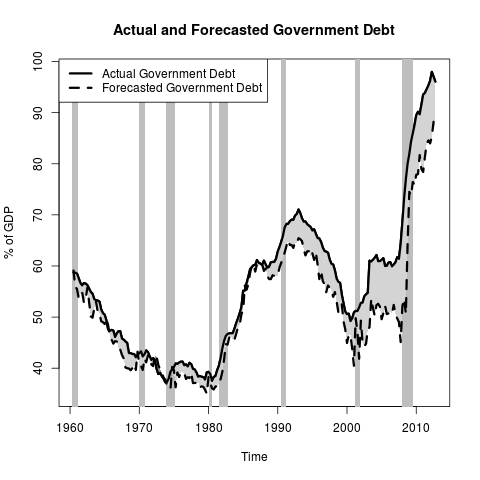
\includegraphics[width=0.45\textwidth, height=0.45\textheight]{pics/pred_debt.png} 
  \end{tabular}
}

\frame
{
  \ft{Fiscal Policy - Prediction Error}
  \begin{tabular}{cc}
    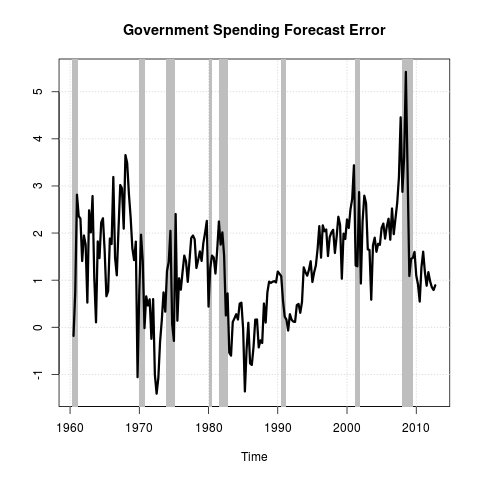
\includegraphics[width=0.45\textwidth, height=0.45\textheight]{pics/fe_gov.png} & 
    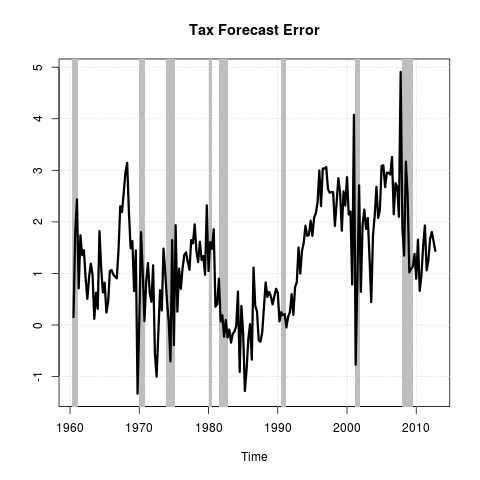
\includegraphics[width=0.45\textwidth, height=0.45\textheight]{pics/fe_tax.png} \\ 
    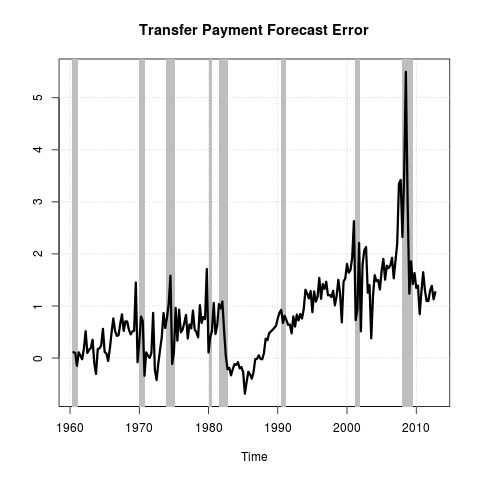
\includegraphics[width=0.45\textwidth, height=0.45\textheight]{pics/fe_transfers.png} & 
    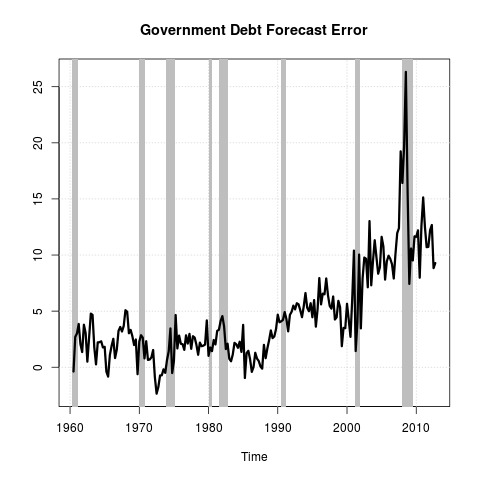
\includegraphics[width=0.45\textwidth, height=0.45\textheight]{pics/fe_debt.png} 
  \end{tabular}
}

\frame
{
  \ft{Fiscal Policy Uncertainty}
  \begin{tabular}{cc}
    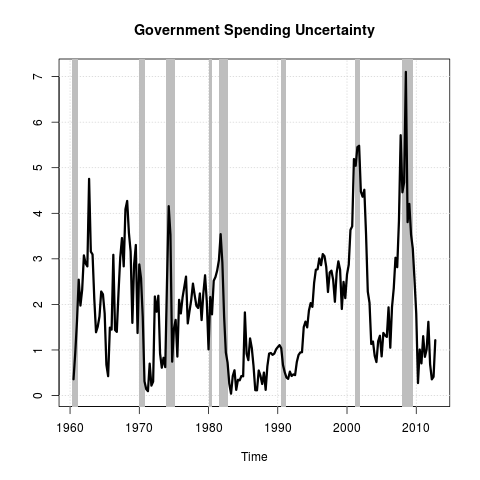
\includegraphics[width=0.45\textwidth, height=0.45\textheight]{pics/fpu_gov.png} & 
    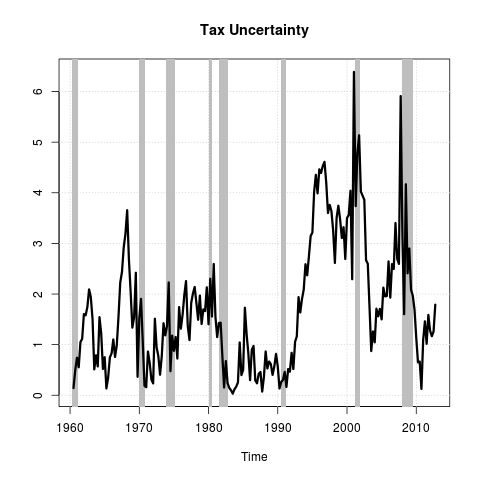
\includegraphics[width=0.45\textwidth, height=0.45\textheight]{pics/fpu_tax.png} \\ 
    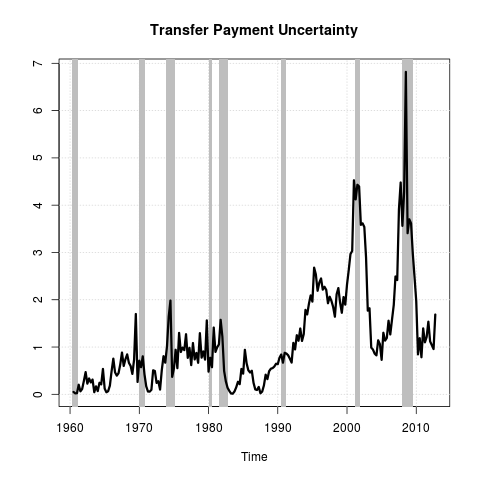
\includegraphics[width=0.45\textwidth, height=0.45\textheight]{pics/fpu_transfers.png} & 
    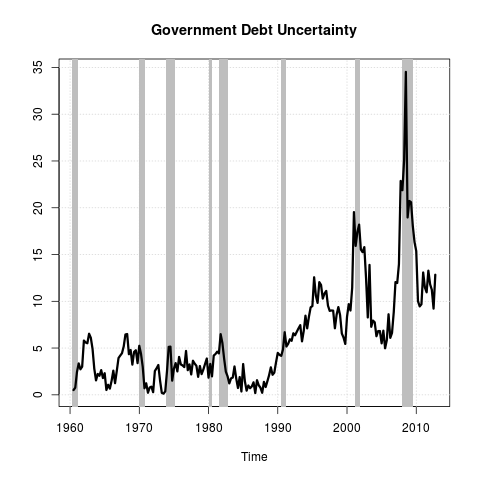
\includegraphics[width=0.45\textwidth, height=0.45\textheight]{pics/fpu_debt.png} 
  \end{tabular}
}

\frame
{
  \ft{Casual Observations}
  \bi
  \item Uncertainty concerning transfers and debt reached unprecedented levels during Great Recession.
    \bi
    \item Government expenditures uncertainty: Nearly 7\% of GDP
    \item Tax uncertainty: Nearly 6\% of GDP
    \item Transfers uncertainty: Nearly 7\% of GDP
    \item Government debt uncertainty: Nearly 35\% of GDP
    \ei
  \item Uncertainty seems to run up for several years preceding recessions:
    \bi
    \item Early 1980s, 2001, 2007.
    \item Not the rule though (eg: declines prior to 1970s, little volatility prior to 1991)
    \ei
  \ei
}

\frame
{
  \ft{Fiscal Uncertainty Correlations}
\begin{scriptsize}
\begin{center}
\textbf{Pearson Correlation Coefficient} \\ \ \\
\begin{tabular}{l|cccc}
 & Gov Spending & Tax Revenue & Transfers & Government Debt \\ \hline
Gov Spending & 1.00 & - & - & - \\
Tax Revenue & 0.75 & 1.00 & - & - \\
Transfers & 0.74 & 0.78 & 1.00 & - \\
Government Debt & 0.64 & 0.65 & 0.90 & 1.00 \\ \hline
\end{tabular}
\end{center}
\end{scriptsize}
\bi
\item All highly correlated. 
\item Common (latent) factor?
\ei
}

\frame
{
  \ft{Fiscal Uncertainty Coincident Indicator}
  \begin{block}{Objective}
    \bi 
    \item Strip out the common component of fiscal uncertainty
    \item Construct a general measure of fiscal uncertainty
    \item Take care of potential multicolinearity problem
    \item Compare to Baker, Bloom, and Davis (2013) (BBD)
    \ei
  \end{block}    

  \begin{block}{Stock and Waston (1989) coincident indicator model}
  \bi
  \item Latent variable: General fiscal uncertainty
    
    \vspace*{-0.5pc} \bdm \begin{array}{l} m_t = m_0 + A \lambda_t + e_t \\ [0.2pc]
\lambda_t = b_1 \lambda_{t-1} + b_2 \lambda_{t-2} + \upsilon_t\\ [0.2pc]
e_t = C e_{t-1} + \eta_t \end{array} \edm
     \vspace*{-0.5pc} \bi
     \item $m_t$: 4x1 vector of fiscal uncertainty variables
     \item $\lambda_t$: general fiscal uncertainty
     \item $m_0 + e_t$: ``unique'' component of fiscal uncertainty.
     \ei
   \ei
   \end{block}
}

\frame
{
  \ft{Coincident Indicator: General Fiscal Uncertainty}
  \begin{center}
    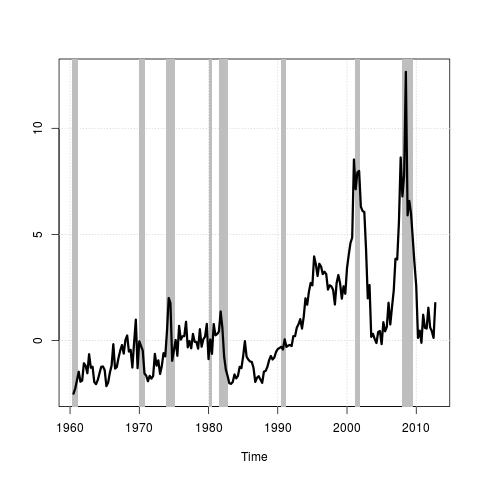
\includegraphics[width=0.8\textwidth]{pics/fpucoin.png}
  \end{center}
}

\frame
{
  \ft{``Unique'' Fiscal Policy Uncertainty}
  \begin{tabular}{cc}
    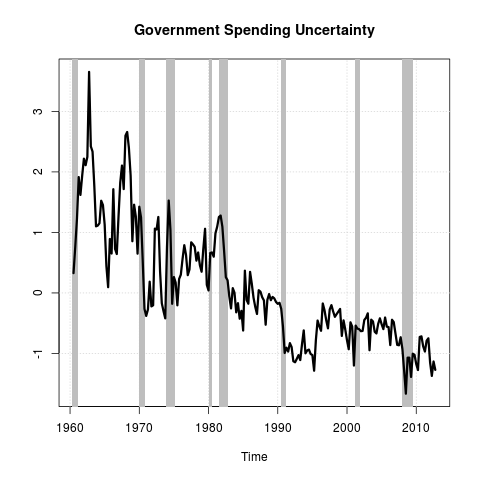
\includegraphics[width=0.45\textwidth, height=0.45\textheight]{pics/fpucoin_gov.png} & 
    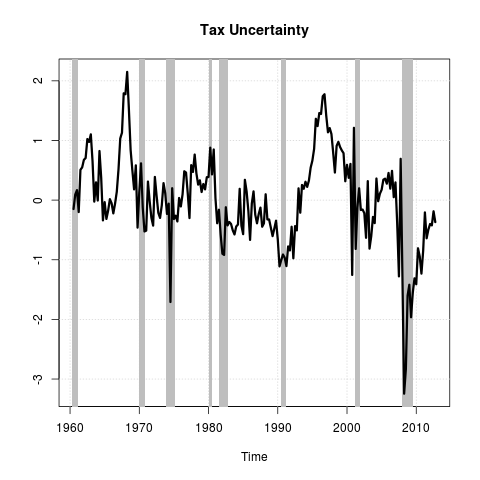
\includegraphics[width=0.45\textwidth, height=0.45\textheight]{pics/fpucoin_tax.png} \\ 
    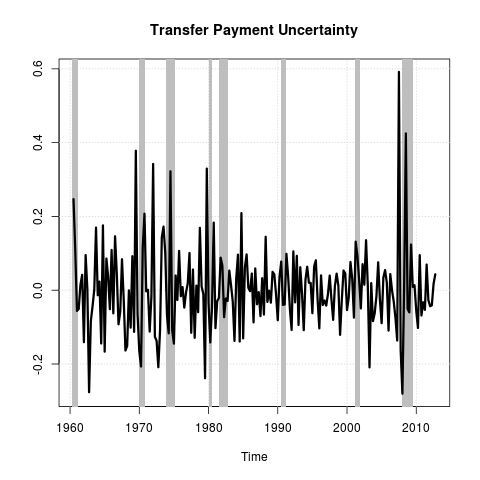
\includegraphics[width=0.45\textwidth, height=0.45\textheight]{pics/fpucoin_transfers.png} & 
    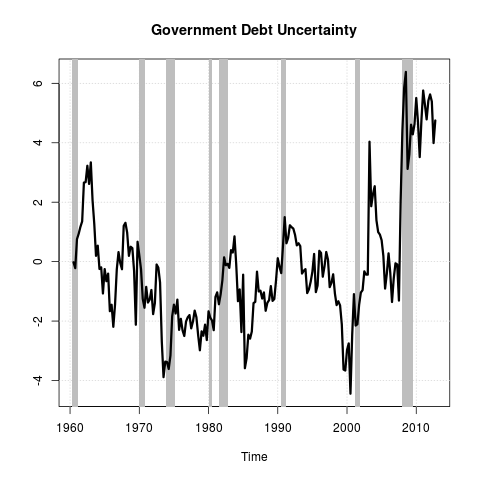
\includegraphics[width=0.45\textwidth, height=0.45\textheight]{pics/fpucoin_debt.png} 
  \end{tabular}
}

\frame
{
  \ft{Fiscal Uncertainty Correlations Redux}
\begin{scriptsize}
\begin{center}
\textbf{Fiscal Uncertainty with Common Component Removed - Pearson Correlations}\\ \ \\
\begin{tabular}{l|cccc}
 & Gov Spending & Tax Revenue & Transfers & Government Debt \\ \hline
Gov Spending & 1.00 & - & - & - \\
Tax Revenue & 0.40 & 1.00 & - & - \\
Transfers & -0.17 & -0.23 & 1.00 & - \\
Government Debt & -0.21 & -0.32 & -0.18 & 1.00 \\ \hline
\end{tabular}
\end{center}
\end{scriptsize}
\ \\ \ \\

\begin{scriptsize}
\begin{center}
\textbf{Correlation of RMSE with Coincident Index}\\ \ \\
\begin{tabular}{l|cccc}
 & Gov Spending & Tax Revenue & Transfers & Government Debt \\ \hline
Coincident Index~ & 0.75 & 0.78 & 0.99 & 0.91 \\ \hline
\end{tabular}
\end{center}
\end{scriptsize}
}

\frame
{
  \ft{Relationship with Baker et. al. (2013)}
\begin{footnotesize}
\hspace*{-2pc}\begin{tabular}{ccc}
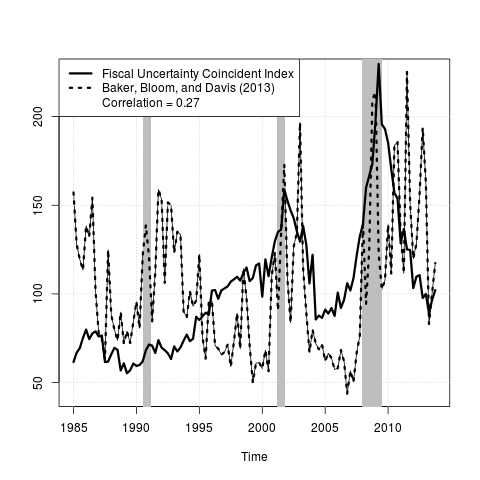
\includegraphics[scale=0.22]{./results/pics0.01/fpuindex.png} & 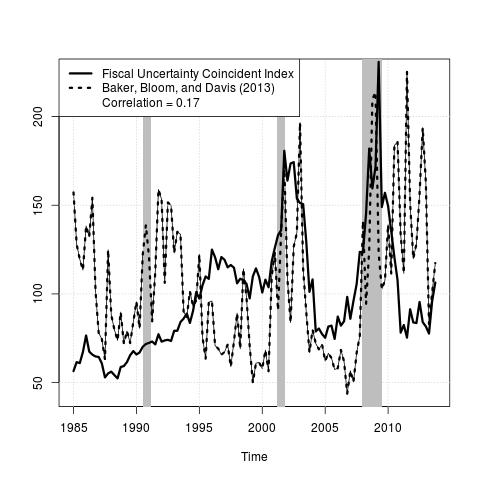
\includegraphics[scale=0.22]{./results/pics0.02/fpuindex.png} & 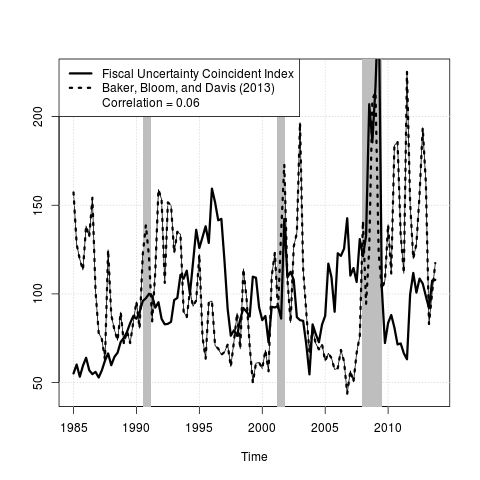
\includegraphics[scale=0.22]{./results/pics0.04/fpuindex.png} \\
Learning Gain = 0.01 & Learning Gain = 0.02 & Learning Gain = 0.04  \\
Correlation = 0.27 & Correlation = 0.17 & Correlation = 0.06 \\
\end{tabular}
\bi
\item Close match post-2000
\item Higher correlation with more empirically plausible learning gains
\item BBD - Headline news is likely endogenous
\item BBD - Tax policy expiration is forward looking
\item BBD is a general economic policy uncertainty index
\ei
\end{footnotesize}
}

\frame[shrink]
{
  \ft{Autoregressive Distributed Lag Model}
  \begin{footnotesize}
  \begin{block}{Dependent Variables: Macroeconomic Outcomes}
    \vspace*{-0.5pc}\begin{columns}
      \column{0.3\textwidth}
      \bi \item Real GDP \item Consumption  \ei
      \column{0.3\textwidth}
      \bi \item Investment \item Inflation \ei 
      \column{0.3\textwidth}
      \bi \item Employment \item Unemployment \ei
      \column{0.05\textwidth}~
    \end{columns}
  \end{block}

  \begin{block}{Key Explanatory Variables: Fiscal Uncertainty Variables}
      \vspace*{-0.5pc}\begin{columns}[t]
      \column{0.45\textwidth}
      \bi \item Government Exp (unique) \item Tax Receipts (unique) \item Transfer Payments (unique) \ei
      \column{0.45\textwidth}
      \bi \item Government Debt (unique) \item Coincident Index \ei ~~~(First lag to avoid endogeneity)
      \column{0.05\textwidth}~
    \end{columns}
  \end{block}

  \begin{block}{Controls}
    \bi 
    \item Lags of all the dependent variables in every model.
    \item Lags of all the fiscal policy variables
    \ei
  \end{block}

  \begin{block}{Specifications}
    \bi
    \item Lag lengths = 1, 2, and 4
    \item Learning gain parameters: 0.01, 0.02, and 0.04
    \ei
  \end{block}

  \end{footnotesize}
}

\frame
{
  \ft{ARDL Results}

\begin{tiny}
\begin{center}
\begin{tabular}{l|S[table-format=3.2] S[table-format=3.2] S[table-format=3.2] S[table-format=3.2] S[table-format=3.2] S[table-format=3.2]}
\textbf{Fiscal Uncertainty} & \multicolumn{6}{c}{\textbf{Dependent Variables (Column Headings)}} \\
\textbf{ - Row Headings -}                 & \multicolumn{1}{p{0.4in}}{\vspace*{-1.5pc}\begin{center}~\newline Real GDP\end{center}} 
                & \multicolumn{1}{p{0.4in}}{\vspace*{-1.5pc}\begin{center}Consumption\end{center}} 
                & \multicolumn{1}{p{0.4in}}{\vspace*{-1.5pc}\begin{center}~\newline Investment\end{center}} 
                & \multicolumn{1}{p{0.4in}}{\vspace*{-1.5pc}\begin{center}Employment\end{center}}
                & \multicolumn{1}{p{0.4in}}{\vspace*{-1.5pc}\begin{center}Unemployment\end{center}} 
                & \multicolumn{1}{p{0.4in}}{\vspace*{-1.5pc}\begin{center}~\newline Inflation\end{center}} \\ [-0.5pc] \hline
 & \multicolumn{6}{c}{} \\ [-0.25pc]
 Government Exp \hl{3} & -0.04 & 0.06 & -0.06 & -0.68** \hl{3} & 0.55*** \hl{3} & 0.02 \\
 (Standard Error) \hl{3} & (0.11) & (0.07) & (0.08) & (0.28) \hl{3} & (0.13) \hl{3} & (0.25) \\ [0.2pc]
 Tax Receipts \hl{5} & 0.36*** \hl{5} & 0.07  & 0.26*** \hl{5} & 0.39 & -0.22 & 0.05 \\
 (Standard Error) \hl{5} & (0.11) \hl{5} & (0.06) & (0.09) \hl{5} & (0.28) & (0.14) & (0.15) \\ [0.2pc]
 Transfer Payments \hl{3} & -0.01 & -0.03 & 0.01 & -0.49** \hl{3} & 0.19*** \hl{3}  & 0.01 \\
 (Standard Error) \hl{3} & (0.08) & (0.04) & (0.04) & (0.23) \hl{3}  & (0.06) \hl{3} & (0.12) \\ [0.2pc]
 Government Debt \hl{4}  & 0.05 & -0.03 & 0.09 & -1.27 \hl{4} & 0.25 \hl{4} & 0.12 \\
 (Standard Error) \hl{4}  & (0.10) & (0.06) & (0.06) & (0.88) \hl{4} & (0.16) \hl{4} & (0.17)  \\ [0.2pc]
 Coincident Index \hl{2} & -0.41*** \hl{2} & -0.21*** \hl{2} & -0.19*** \hl{2} & 0.13 & -0.22* & -0.36** \hl{2} \\
 (Standard Error) \hl{2} & (0.10) \hl{2} & (0.05) \hl{2} & (0.07) \hl{2} & (0.38) & (0.14) & (0.16) \hl{2} \\ [0.2pc]
\hline
 & \multicolumn{6}{c}{} \\ [-0.25pc]
Joint Wald & 4.02*** & 3.80*** & 2.54** & 3.21*** & 4.27*** & 1.29 \\ [0.25pc] \hline

 & \multicolumn{6}{c}{} \\ [-0.25pc]
 Adjusted R-square & 0.32 & 0.98 & 0.96 & 0.83 & 0.87 & 0.81 \\
 AIC & 466.15 & 198.35 & 257.72 & 666.99 & 398.54 & 632.69 \\
 BIC & 549.83 & 282.03 & 341.40 & 750.67 & 482.22 & 716.37 \\ \hline

\end{tabular}

\end{center}
\end{tiny}
\begin{scriptsize}
\only<1>{~ \\  ~ \\ }
\only<2>{\textcolor{BrickRed}{\textbf{1. Common fiscal uncertainty dampens aggregate demand}}}
\only<3>{\textcolor{BrickRed}{\textbf{2. Transfers and Gov Exp uncertainty drags on employment}}}
\only<4>{\textcolor{BrickRed}{\textbf{3. Debt uncertainty drags on employment (significant in most other specifications)}}}
\only<5>{\textcolor{BrickRed}{\textbf{4. Tax uncertainty boosts investment and real GDP}}}
\end{scriptsize}
}

\frame
{
  \ft{Magnitude of the Impact}
  \bi
  \item Fern\'andez-Villiverde et. al. (2011): Fiscal uncertainty is a ``once-in-a-decade'' concern
  \item Baker, Bloom, and Davis (2013): Build-up of uncertainty from 2006-2011
  \item Focus on general fiscal uncertainty (coincident index)
    \bi
    \item Find when it is highest - 2009:Q2 (with all learning gains)
    \item Find quarter in decade preceding when it was lowest - 2005:Q4
    \item Change in macroeconomic activity attributed to this buildup
    \ei
  \ei
}

\frame
{
  \ft{Magnitude of the Impact}
\begin{scriptsize}
\begin{center}
\textbf{Magnitude of Extreme Change in Coincident Fiscal Uncertainty}\\
\textbf{(Learning Gain = 0.02)} \\
~ \\
\begin{tabular}{l|S[table-format=3.2] S[table-format=3.2] S[table-format=3.2] S[table-format=3.2]} \hline
\multicolumn{3}{l}{Largest Value Coincident Fiscal Uncertainty = 4.77} & \multicolumn{1}{r}{Date: 2009 Quarter 2} & \\
\multicolumn{3}{l}{Smallest Value in Decade Preceding = -0.34} & \multicolumn{1}{r}{Date: 2005 Quarter 4} & \\ \hline
\end{tabular} \\
~ \\
~ \\
\textbf{Estimated Impact - ARDL(2)} \\
~ \\
\begin{tabular}{l|S[table-format=3.2] S[table-format=3.2] S[table-format=3.2] S[table-format=3.2]}
 \multicolumn{1}{p{0.85in}}{Variable} 
                & \multicolumn{1}{p{0.85in}}{\vspace*{-1.5pc}\begin{center}Impact\end{center}} 
                & \multicolumn{1}{p{0.85in}}{\vspace*{-1.5pc}\begin{center}95\% Lower Bound\end{center}} 
                & \multicolumn{1}{p{0.85in}}{\vspace*{-1.5pc}\begin{center}95\% Upper Bound\end{center}}\\ [-0.75pc] \hline
Real GDP &  -2.07*** & -3.04 & -1.11 \\
Consumption &  -1.06*** & -1.57 & -0.54 \\
Investment &  -0.96*** & -1.64 & -0.29 \\
Employment &  0.65 & -3.15 & 4.45 \\
Unemployment & -1.14* & -2.49 & 0.21 \\
Inflation & -1.85** & -3.50 & -0.20 \\
\hline
\end{tabular}
\end{center}
\end{scriptsize}
}


\frame
{
  \ft{Conclusions}
  Fiscal Uncertainty Reduces Economic Activity

  \bi
  \item General measure for fiscal uncertainty associated with:
    \bi
    \item lower real GDP,
    \item lower consumption,
    \item lower investment.
    \ei
 
  \item Uncertainty regarding specific fiscal variables 
    \bi
    \item Government expenditures, transfer payments, and government debt associated with reductions in employment / increases in unemployment
    \item Tax uncertainty associated with increases in investment and real GDP
    \ei

  \item General fiscal uncertainty significant drag during the Great Recession:
    \bi
    \item Responsible for a 1\% to 3\% decrease in real GDP
    \item Decreased consumption by about 1\% of real GDP
    \item Decreased investment by about 1\% of real GDP
    \ei
  \ei
}








\end{document}

